\achapter

\stepcounter{answer}
\answer 取$ x $轴沿飞机航向,$ y $轴竖直地指向地面

(1) 取发射点为原点,炮弹轨迹方程为

$    y = \dfrac { g x ^ { 2 } } { 2 \left( v _ { 0 } + v \right) }$


(2) 取发射点为原点,炮弹轨迹方程为

$    y = \dfrac { g x ^ { 2 } } { 2 v ^ { 2 } }$

(3) 取炮弹质心为原点,飞机发射点之轨迹方程为

$    y = - \dfrac { g x ^ { 2 } } { 2 v ^ { 2 } }$

\answer $ | \vec{v} | = 2 1 . 6   $公里,与水平的车行方向夹角为 $ \theta = 7 3 ^ { \circ } 5 4 ^ { \prime }   $,如图所示
\begin{figure}[h]
    \vspace{-0.8em}
    \centering
    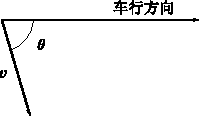
\includegraphics{figure/figa02.01}
    \caption{}
    \label{figa:02.01}
    \vspace{-0.8em}
\end{figure}

\stepcounter{answer}
\answer 水流速率$  v = 5 . 0   $公里/时

\answer (1) $ \varphi _ { 1 } = tg ^ { - 1 } \dfrac { v _ { 0 } } { v _ { 1 } }   $

(2) $ \varphi _ { 2 } = \tg ^ { - 1 } \dfrac { v _ { 0 } } { t _ { 1 } + v _ { 2 } }  $

(3) $ v ^ { \prime } = \sqrt { v _ { 1 } ^ { 2 } + v _ { 2 } ^ { 2 } }, v'' = \sqrt { \left( v _ { 1 } + v _ { 2 } \right) ^ { 2 } + v _ 0 ^ { 2 } }  $

\answer (1) $ | \vec{v} | = \sqrt { u ^ { 2 } + {v'} ^ { 2 } } = 2 0 4   $公里/时
\begin{equation*}
    \alpha = \tg ^ { - 1 } \frac { u } { v' } = 1 1^\circ 30'
\end{equation*}

(2) $ | \vec{v} | = \sqrt { {v'} ^ { 2 } - u ^ { 2 } } = 1 9 5 . 9 6 \approx 196 $公里/时
\begin{equation*}
    \theta = \sin ^ { - 1 } \dfrac { u } { v } = 1 1 ^ { \circ } 3 0 '
\end{equation*}\vspace{-1.3em}
\begin{figure}[h]
    \centering
    \subfigure[]{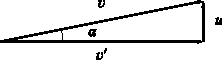
\includegraphics{figure/figa02.02a}}
    \qquad
    \subfigure[]{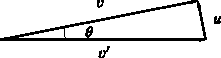
\includegraphics{figure/figa02.02b}}
    \caption{}
    \label{figa:02.02}
\end{figure}\vspace{-1em}

\answer $ t _ { 0 } = \dfrac { 2 L } { u } $

% 381.jpg

(1) $ t _ { 1 } = \dfrac { t _ { 0 } } { 1 - v ^ { 2 } \operatorname{/} u ^ { 3 } }   $

(2) $ t _ { 2 } = \dfrac { t _ { 0 } } { \sqrt { 1 - v ^ { 2 } \operatorname{/} u ^ { 2 } } }  $\vspace{-1em}

(3) $t_{3}=\dfrac{t_{0}}{\sqrt{1-\dfrac{v^{2}}{u^{2}} \sin ^{2} \theta \Big[1-\dfrac{v^{2}}{u^{2}}\cdot \dfrac{\cos^2\theta}{ 1-\left(v^{2} \operatorname{/} u^{2}\right) \sin ^{2} \theta}\Big]}}$

\answer $ t = 0 . 3 7 $ 秒,与参考系的选取无关

\answer $ \theta = \tg ^ { - 1 } \dfrac { 2 g h } { v }   $

\answer  $ 5 \times 1 0 ^ 8$年

\answer (1) $ v _ { A B } = v _ { A } + v _ { B }  $

(2) $ v _ { A B } = 1 . 4 c $

(3) 不违反。狭义相对论只是说,在任一惯性系中,光速不变。换一
句话说,即:若以此两物之一为参考系,要知另一物的速度就要用相
对论的速度合成公式

(4) $ v ^ \prime _ { B } \ne v _ { A B } $

\answer (1) $ 0.87 l $

(2) $ 1 . 1 5 \Delta t $

\answer $ v = 0 . 9 9 9 8 c   $

\answer $  \Delta \tau _ \text{赤极} = 1 . 8 8 4 3 \times 1 0 ^ { 5 } \text{秒} = 2 . 1 8 0 9  \text{天}= 5 . 9 7 5 0 \times 1 0 ^ { - 3 } \text{年} $

\answer $  \Delta \tau _ \text{月地} = 9.12 \times 1 0 ^ { 5 } \text{秒} = 10.55  \text{天}= 2.89 \times 1 0 ^ { - 2 } \text{年} $

\answer $  \Delta \tau _ \text{日地} = 7.75 \times 1 0 ^ { 5 } \text{秒} = 8.979 \text{天}= 2.46 \times 1 0 ^ { - 2 } \text{年} $

\answer $ \tau = \dfrac { \tau _ 0 } { \sqrt{ 1 - v ^ { 2 } \operatorname{/} c ^ { 2 } } } $

\answer $ \tau = 1 0 \tau _ { 0 } = 2 2   $微秒
